
\section{Signal processing programs}

% pv-change: \subsection{Seicmic Handler}
% pv-change: \subsection{MatSeis}

The two processing systems PITSA\index{PITSA} and SAC\index{SAC} are interfaced to SEISAN and can be started directly from EEV. This is done since both systems support functions that SEISAN does not have. They only operate on Unix. The Degtra program only operates in Windows. It is not interfaced directly to SEISAN but operates on SEISAN format. 

\subsection{PITSA}
\label{subs:pitsa}

PITSA (Programmable Interactive Toolbox for Seismological Analysis) 
is a program written by \textbf{Frank Scherbaum} and \textbf{James Johnson}. The program 
is included in the SEISAN package, updated versions are available at 
\url{http://lbutler.geo.uni-potsdam.de/service.htm}. From this version, 
PITSA is interfaced with the SEISAN system through the program WAVETOOL, 
which converts waveform files from SEISAN to the GSE2 format. PITSA 
since version 5.0 supports reading multi channel GSE2 files. PITSA 
can be started from EEV by typing `pitsa' on the prompt line. All 
waveform files listed in the S-file will be converted to multi-channel 
GSE2 files.  The multi-converted files are put into your local directory 
and are named `gse1', `gse2' etc. The response is converted to GSE format. 
When PITSA is started, the waveform files have to be loaded using 
the GSE2 input format. The response file names will be given as 
described in the GSERESP section.  

\subsection{SAC2000}


SAC2000 (seismic analysis code) is currently developed by \textbf{Lee Minner} and \textbf{Peter Goldstein} \citep{goldstein1999}. SAC is not distributed with SEISAN, information on SAC can be obtained from the SAC homepage (\url{http://www-ep.es.llnl.gov/www-ep/esd/seismic/sac.html}). The main features of SAC include general arithmetic operations, Fourier transforms, three spectral estimation techniques, IIR and FIR filtering, signal stacking, decimation, interpolation, correlation, and seismic phase picking. SAC also contains an extensive graphics capability. 
With SAC it is possible to write macros, which helps to process large amounts of data. The SAC format is used in several research oriented programs. SAC can be started from EEV using the command `sac'. EEV will start the WAVETOOL program to convert the data to SAC and then execute the command sac. In case your sac executable is called sac2000, it is necessary to rename it (to sac) or alternatively to create a link in either the SEISAN PRO directory or the SAC bin directory. This is done for example by the command :\newline
\texttt{ln -s /sac/bin/sac2000 /sac/bin/sac} \newline 
Since the SAC format is a single trace format, the SEISAN multichannel files are split into single trace files. The station and component names are included in the file name and the suffix `SAC' is added to all SAC files. 
For both systems, waveform data can be converted to the respective format outside EEV using WAVETOOL, GSESEI or SACSEI, and the programs can be started without using EEV. 

\subsection{Degtra A4}


Degtra A4 is a Windows-based computer system designed to process 
ground-motion time histories for seismology, engineering seismology 
and earthquake engineering applications. It has been developed at 
the Institute of Engineering, UNAM, Mexico, where it has been used 
as a professional and teaching tool for more than 10 years. 
Figure \ref{fig:degtra} shows a typical view of Degtra A4. 

\begin{figure}
\htmlimage{scale=2.0}
\centerline{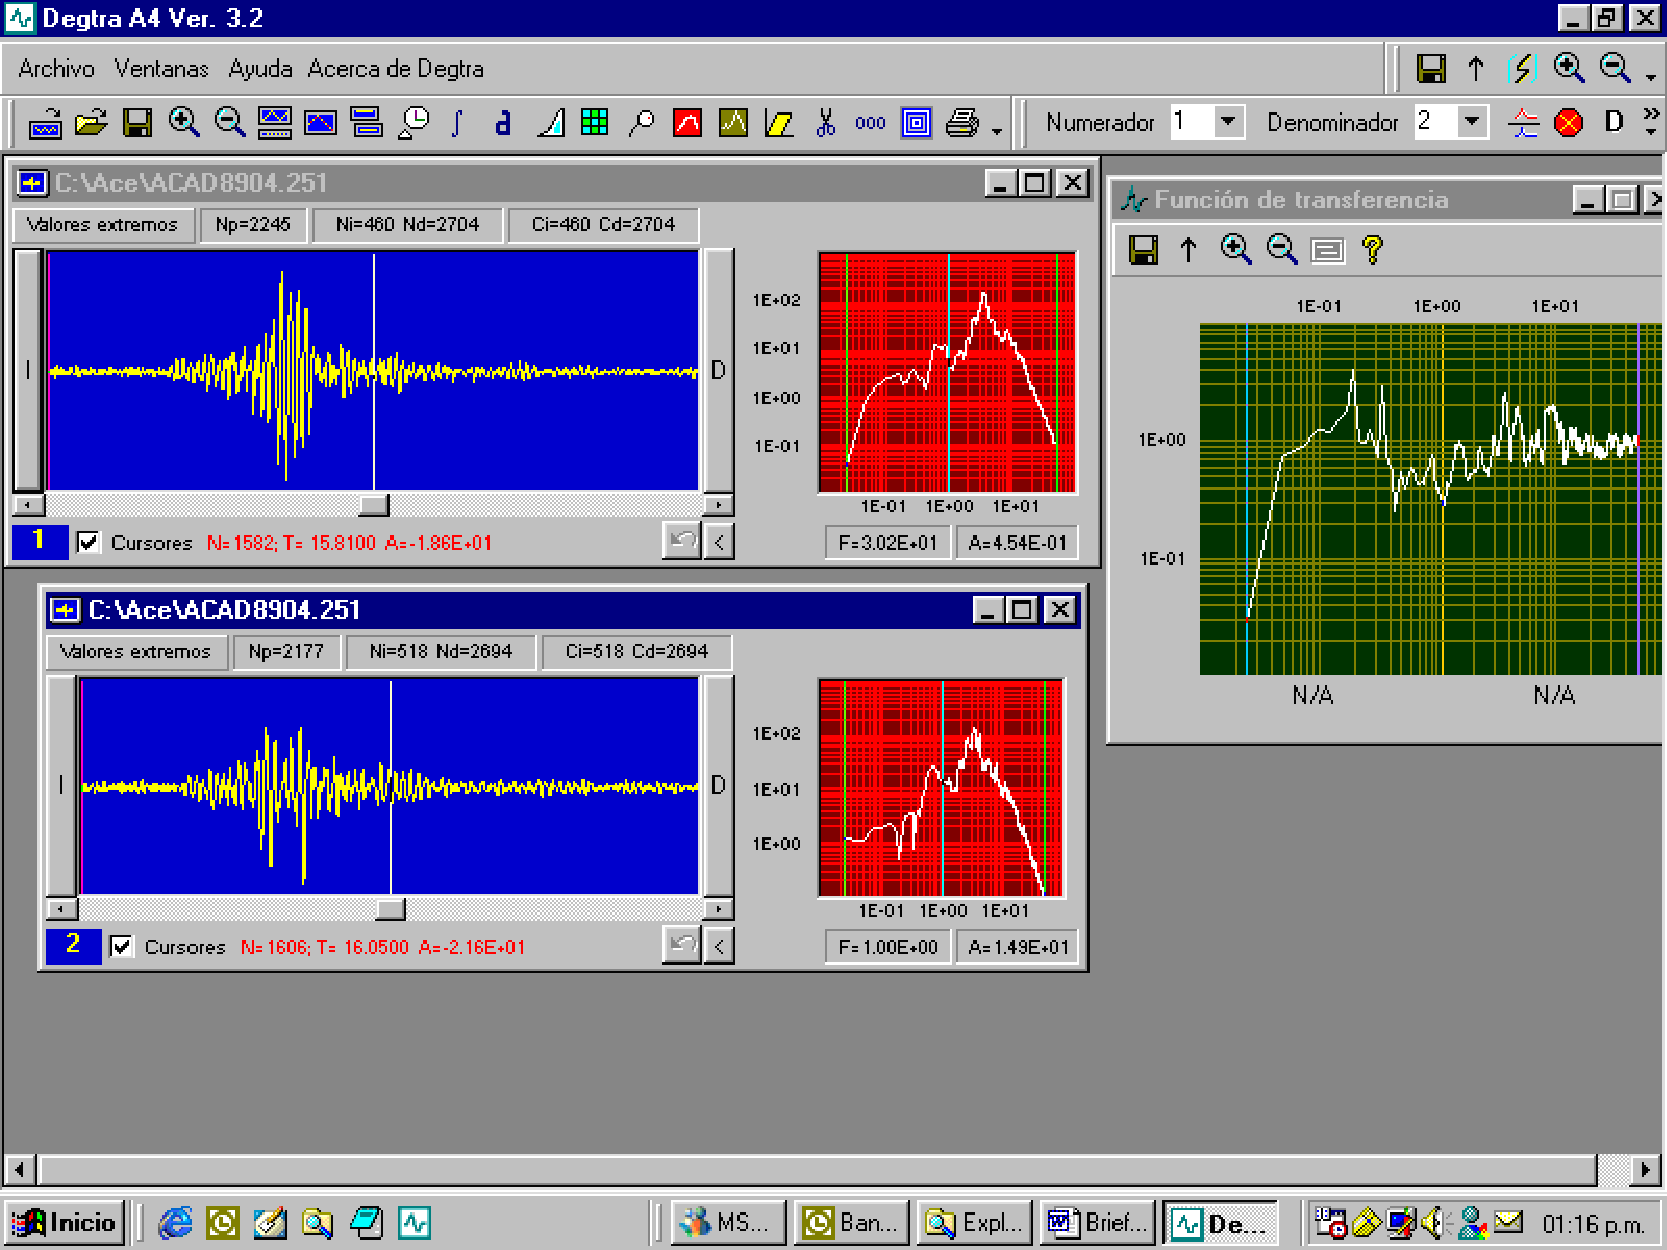
\includegraphics[width=0.9\linewidth]{fig/fig36}}
\caption{Example of DEGTRA A4.}
\label{fig:degtra}
\end{figure}

Degtra A4 accepts input ground-motion recordings written in several formats: simple ASCII or binary files, SEISAN format and the standard format of the Mexican Strong-Motion Database. 

The program has a nice and user-friendly interface, in which several time-histories can be manipulated at a time. It includes zoom-in/zoom-out capabilities that can be used if only a portion of a recording is of interest. 

There are two types of operations that Degtra A4 can perform using strong-motion recordings: operations involving a single recording and operations involving two recordings. 

Among the first group, the main functions are the following: 

\begin{itemize}
\item
Scaling. Multiplies the recording by a constant 
\item
Decimation. Decimates the recording by a user-given factor 
\item
Base-line correction: Includes several methods. 
\item
Differentiation: Numerical differentiation with respect to time. 
\item
Integration: Numerical integration with respect to time. 
\item
Computation of Arias' intensity. 
\item
Filtering: Includes high-pass, low-pass, band-pass and band-stop Butterworth filters, as well as Gaussian and Futterman filters. 
\item
Computation of elastic response spectra. Computes absolute acceleration, relative velocity, relative displacement and pseudo acceleration response spectra. 
\item
Computation of inelastic response spectra. Computes required-strength response spectra for fixed ductility demand of bilinear systems. 
\item
Computation of Fourier spectra. Computes and (optionally) smoothes FFT of a time signal. 
\item
Computation of response (acceleration, velocity, displacement) of elastic and inelastic (bilinear) single-degree-of-freedom oscillators. 
\item
Computation of the S-wave response of a soil column of given properties assuming that the time-history is the incident wave field at the base of the column. 
\end{itemize}


The main operations involving two recordings are: 
\begin{itemize}
\item[-]
 Spectral ratio. Computes the (Fourier) spectral ratio between two recordings. 
\item[-]
Odogram. Displays an X-Y parametric representation (time is the parameter) of two recordings, typically ground displacements, in order to observe particle trajectories. 
\item[-]
Addition/Difference. Computes the sum or difference of two recordings. This is useful, for instance, to identify rocking or torsional motions in buildings. 
\item[-]
Rotation: Rotates two components of the ground motion to arbitrary angles. 
\item[-]
Cross-correlation: Computes cross-correlation between two signals. 
\item[-]
Coherence: Computes coherence between two signals. 
\end{itemize}

Degtra A4 includes an on-line help file with details about the meaning of required parameters, techniques used, and use of Degtra A4 itself. It is available in two versions: one for Windows 2000 or lower and another for Windows XP. Installation is made with a typical Windows executable setup file. The distribution is found in directory SUP. 

Degtra A4 is currently in Spanish, English version in preparation. 

For questions please contact: 

\textbf{Mario Ordaz}, Institute of Engineering, UNAM \newline
mors@pumas.iingen.unam.mx 

